\documentclass[conference]{IEEEtran}
\IEEEoverridecommandlockouts % needed for \thanks in IEEE conference mode

\usepackage[utf8]{inputenc}
\usepackage[T1]{fontenc}
\usepackage{hyperref}
\usepackage{url}
\usepackage{booktabs}
\usepackage{amsfonts}
\usepackage{amsmath}
\usepackage{amssymb}
\usepackage{graphicx}
\usepackage{xcolor}
\usepackage{multirow}
\usepackage{cite}
\usepackage{balance}
\usepackage{tikz}
\usetikzlibrary{arrows.meta,positioning,calc}

\hypersetup{
  colorlinks=true,
  linkcolor=blue,
  citecolor=blue,
  urlcolor=blue,
}

\begin{document}

\title{Does Sentiment Fusion Help?\\A Selection-Bias-Free Re-Evaluation of Multimodal Stock Movement Prediction}

% TODO (authors): verify full given names before camera-ready. 
\author{
\IEEEauthorblockN{
Donghao HUANG\textsuperscript{1,2},
Zheng Kai HENG\textsuperscript{2},
Zhaoxia WANG\textsuperscript{2,*}
\thanks{*Corresponding author: zxwang@smu.edu.sg}
}
\IEEEauthorblockA{\textsuperscript{1}Research and Development, Mastercard, Arlington, VA, USA}
\IEEEauthorblockA{\textsuperscript{2}School of Computing and Information Systems, Singapore Management University, Singapore}

\IEEEauthorblockA{
donghao.huang@mastercard.com;
zkheng.2023@scis.smu.edu.sg;
zxwang@smu.edu.sg
}
}
\maketitle

\begin{abstract}
Multimodal stock-movement prediction---fusing financial-news and social-media
sentiment with technical indicators---is widely reported to deliver large
risk-adjusted gains, with recent studies citing average Sharpe ratios above
two. We show that such gains are, to a substantial degree, artifacts of
optimistic evaluation rather than evidence that sentiment fusion works. We
build a selection-bias-free evaluation protocol for multimodal financial
prediction---an explicit chronological train/validation/test split with an
embargo, model and horizon selection locked to the validation window, and
multi-seed reporting with paired significance tests---and apply it to a
comprehensive grid of 4{,}200 task-specific runs (seven model families, eight
feature configurations, five U.S.\ equities, three horizons, five seeds) plus
two time-series foundation models (Chronos-2, FinCast). Three findings emerge.
\emph{First}, selecting the best model and horizon per stock on the test set
inflates the average Sharpe ratio from 1.40 to 2.29---accounting for most of
the headline numbers reported in prior work. \emph{Second}, under bias-free
evaluation a technical-indicator-only baseline is \emph{not} beaten by any
sentiment configuration: fixed 70:30 news--social fusion, equal weighting,
news-only, social-only, and a learned reliability-weighted fusion all
underperform technical-only, by $+0.58$ Sharpe on average for fixed 70:30
($p<10^{-20}$, paired Wilcoxon). \emph{Third}, time-series foundation models do
not beat task-specific models and mostly post negative Sharpe ratios. We
conclude that, in this setting, the reported value of multimodal sentiment
fusion is largely an evaluation artifact, and we release a reproducible
benchmark to support more careful future studies.
\end{abstract}

\begin{IEEEkeywords}
stock movement prediction, multimodal fusion, sentiment analysis, evaluation
methodology, selection bias, backtest overfitting, financial machine learning,
reproducibility
\end{IEEEkeywords}

%===============================================================================
\section{Introduction}

Short-term stock-movement prediction is a long-standing application of data
mining, and the dominant recent paradigm is \emph{multimodal}: combine
quantitative signals (technical indicators derived from price history) with
qualitative signals (sentiment extracted from financial news and social media)
\cite{xu2018,sawhney2020,karadas2025,wang2023learning}. A steady stream of
papers reports that incorporating sentiment produces large, economically
meaningful gains, often summarized by trading metrics: long/short strategies
driven by news sentiment have reported Sharpe ratios above $2.0$ net of
transaction costs~\cite{kirtac2024}.

These reports sit uneasily beside two well-established facts. First, financial
return series have a very low signal-to-noise ratio, and the machine-learning
finance literature has repeatedly documented how easily backtests
\emph{overfit}: with enough models, horizons, and hyperparameter
configurations, a strategy that is indistinguishable from noise can be made to
look excellent purely by selection \cite{bailey2014dsr,bailey2016pbo,prado2018,
arnott2019,harvey2016}. Second, when general-purpose machine-learning methods
are evaluated against simple baselines under disciplined protocols, the
reported advantages frequently shrink or disappear \cite{makridakis2018}.

This paper asks a deliberately narrow, falsifiable question: \emph{under a
selection-bias-free evaluation protocol, does multimodal sentiment fusion
improve short-term stock-movement prediction relative to a technical-indicator
baseline?} We answer it with a comprehensive experimental analysis rather than
a new model. We re-implement a conventional multimodal-fusion pipeline---FinBERT
sentiment, technical indicators, classical and neural classifiers, a long/short
backtest---and evaluate it under a protocol designed to control for selection.
The apparent advantage of fusion does not survive that protocol.

Concretely, we make three contributions.

\begin{itemize}
\item \textbf{A selection-bias-free evaluation protocol} for multimodal
financial prediction (Section~\ref{sec:protocol}): an explicit
train/validation/test chronological split with an embargo gap; \emph{all}
model-family and horizon selection locked to the validation window; multi-seed
training; and reporting with paired significance tests alongside
backtest-overfitting diagnostics \cite{bailey2014dsr,bailey2016pbo}.

\item \textbf{A learned reliability-weighted sentiment fusion} that generalizes
the fixed 70:30 news--social heuristic of prior work \cite{nyakurukwa2024} into
a data-driven, prior-regularized weight estimated on validation data
(Section~\ref{sec:protocol}-D). We report it honestly: it does not help.

\item \textbf{A comprehensive re-evaluation} (Section~\ref{sec:results})
across $4{,}200$ task-specific runs and two time-series foundation models,
yielding three insights: (i)~test-set selection inflates the average Sharpe
ratio from $1.40$ to $2.29$; (ii)~no sentiment configuration beats a
technical-only baseline under bias-free evaluation; (iii)~foundation models do
not beat task-specific models. We release code and the processed benchmark at GitHub\footnote{\url{https://github.com/inflaton/Multimodal-Stock-Movement-Prediction}}.
\end{itemize}

Our intent is not to claim that sentiment is uninformative in all settings, but
to show that a frequently reported positive result does not survive careful
evaluation---a comprehensive experimental analysis that yields new insight into
the strengths and weaknesses of an existing and widely used method.
Fig.~\ref{fig:overview} summarizes the study: a conventional multimodal
pipeline, executed inside a selection-bias-free evaluation protocol.

\begin{figure*}[t]
\centering
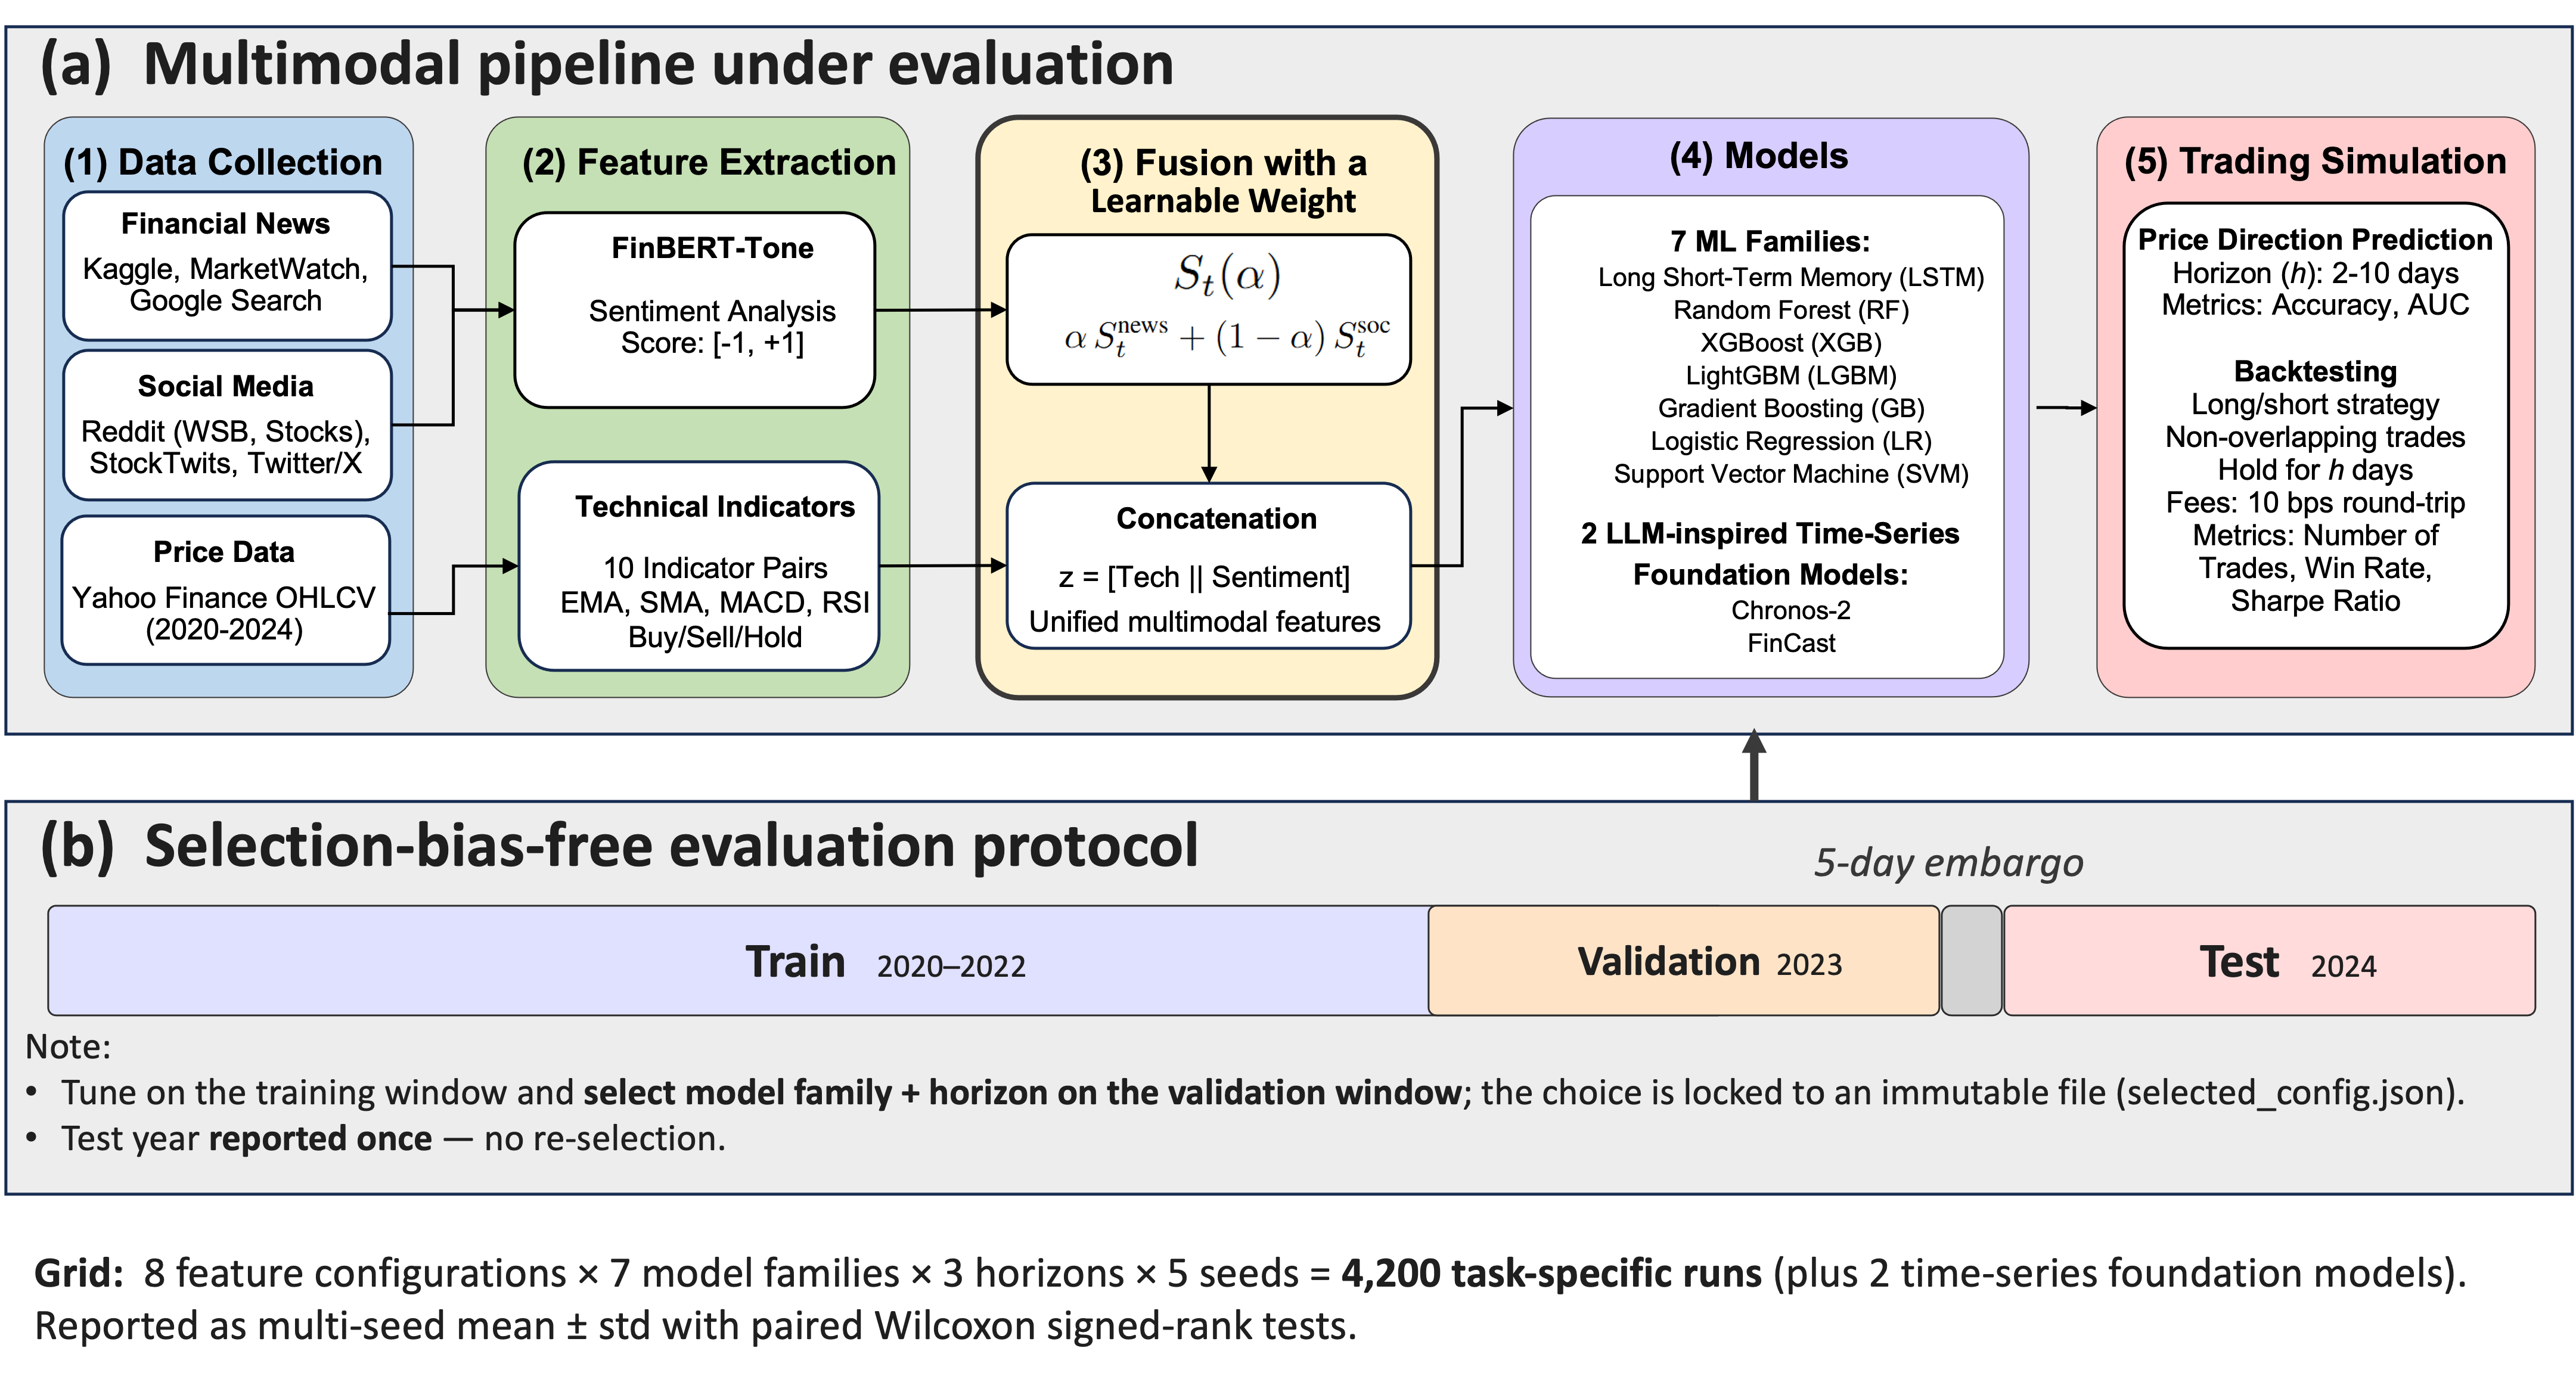
\includegraphics[width=\textwidth]{figures/Figure1.png}
\caption{Overview of the study. (a)~A conventional multimodal stock-movement
pipeline: news, social-media, and price data are turned into FinBERT-Tone
sentiment and technical-indicator features, fused, fed to seven model families,
and evaluated by a long/short backtest. (b)~The selection-bias-free evaluation
protocol that is the methodological contribution: a chronological
train/validation/test split with a five-day embargo; \emph{all} model-family
and horizon selection locked to the 2023 validation window; and a 4{,}200-run
multi-seed grid reported with paired significance tests. Every grid cell is one
execution of pipeline~(a).}
\label{fig:overview}
\end{figure*}

%===============================================================================
\section{Related Work}

\noindent\textbf{Multimodal stock-movement prediction.}
Combining textual sentiment with market data is now standard. StockNet
\cite{xu2018} pairs tweets with prices; MAN-SF \cite{sawhney2020} adds
attentive cross-modal and inter-stock modeling; more recent work fuses news,
social media, and engineered indicators
\cite{karadas2025,wang2023learning,jaggi2021}. Domain-adapted language models
such as FinBERT \cite{araci2019,huang2022} are the usual sentiment extractors.
A recurring design choice is how to weight news against social media:
Nyakurukwa and Seetharam \cite{nyakurukwa2024} report that news sentiment
correlates more strongly with returns, motivating a fixed 70:30
news-to-social weighting that several pipelines adopt. Most of these studies
report sizeable gains for fusion over price- or indicator-only baselines.

\noindent\textbf{Time-series foundation models.}
General-purpose forecasters pre-trained on large, heterogeneous corpora---e.g.,
Chronos-2 \cite{ansari2025chronos} and the finance-specific FinCast
\cite{zhu2025fincast}---offer zero-shot and fine-tuned prediction and can, in
principle, ingest covariates. Whether their broad pre-training transfers to the
noisy, non-stationary regime of equity returns is not well characterized.

\noindent\textbf{Evaluation pitfalls in financial ML.}
The financial-machine-learning literature has long warned that the binding
constraint is evaluation, not modeling. L\'opez de Prado \cite{prado2018}
catalogues leakage and overfitting failure modes; Bailey and L\'opez de Prado
\cite{bailey2014dsr} introduce the Deflated Sharpe Ratio to correct an observed
Sharpe ratio for the number of trials conducted; the Probability of Backtest
Overfitting \cite{bailey2016pbo} quantifies how often an in-sample-best
configuration underperforms out of sample; Harvey et al.\ \cite{harvey2016} and
Arnott et al.\ \cite{arnott2019} document multiple-testing inflation across the
field. Empirical-asset-pricing studies that adopt disciplined protocols
\cite{gu2020} typically report modest, carefully bounded effects. Our
contribution is to bring this discipline to bear specifically on the
\emph{multimodal-fusion} question, and to quantify how much of the reported
advantage it removes.

%===============================================================================
\section{
%Evaluation Protocol
Methodology and Evaluation Protocol}
\label{sec:protocol}

We first state the prediction task, then describe the four elements of the
protocol that distinguish bias-free evaluation from the optimistic evaluation
common in prior work.

\subsection{Problem Formulation}
For a stock $s$ with closing-price series $\{p_t\}$, the binary movement label
at horizon $h$ is
\begin{equation}
y_{t+h} = \mathbb{I}\!\left[\frac{p_{t+h}-p_t}{p_t} > \theta\right],
\end{equation}
where $\mathbb{I}[\cdot]$ is the indicator function and $\theta$ is a
per-(stock,\,horizon) threshold chosen \emph{on the training window} to
balance the two classes. A model receives a feature vector $\mathbf{z}_t$
combining technical indicators $\mathbf{X}_t$ and an aggregated daily sentiment
score $S_t$ (Section~\ref{sec:setup}), and outputs $\hat{p}(y_{t+h}=1)$.
Predictions are evaluated both as a classification problem (ROC-AUC) and
through a long/short trading simulation with non-overlapping $h$-day positions
and $10$\,bps round-trip transaction costs.

\subsection{Chronological Split with Embargo}
All data span January 2020 to December 2024. We use a strict calendar split:
\textbf{training} 2020--2022, \textbf{validation} 2023, \textbf{test} 2024. The
last $h$ rows of the validation window are dropped so that validation labels,
which look $h$ days ahead, cannot reach into the test year, and a further
five-trading-day \emph{embargo} is removed from the start of the test window
\cite{prado2018}. This replaces the train/test-only split of prior pipelines,
which leaves no clean data on which to make modeling choices.

\subsection{Validation-Locked Model and Horizon Selection}
This is the single most consequential element. Prior multimodal pipelines
typically report, for each stock, the \emph{best} model family and prediction
horizon---but the ``best'' is identified on the test year. With seven model
families and nine candidate horizons, that is up to $63$ trials per stock; the
maximum over $63$ noisy trials is a badly upward-biased estimate of true
performance \cite{bailey2014dsr,harvey2016}.

We instead compute, for every (stock, ablation, model, horizon) cell, the
\emph{validation} ROC-AUC and validation Sharpe ratio, and write the
selection---which model and which horizon---to an immutable configuration file
keyed only by validation scores. Every number reported on the 2024 test year
is then read back through that file. No test-set quantity is ever used to make
a modeling choice. Section~\ref{sec:results}-A quantifies how much this single
change removes.

\subsection{Learned Reliability-Weighted Fusion}
Prior work aggregates daily news sentiment $S^{\text{news}}_t$ and social sentiment $S^{\text{soc}}_t$ with fixed weights\cite{nyakurukwa2024}:
\begin{equation}
S_t = 0.7\,S^{\text{news}}_t + 0.3\,S^{\text{soc}}_t, 
\label{eqn:fix-weight}
\end{equation}
%citing the empirical news--return relationship \cite{nyakurukwa2024}. A fixed constant borrowed from another study is a hyperparameter, not a method. 

%We generalize it to a learned weight 
We generalize Equation~\ref{eqn:fix-weight} by introducing a learnable weight:
\begin{equation}
S_t(\alpha) = \alpha\,S^{\text{news}}_t + (1-\alpha)\,S^{\text{soc}}_t%,
\end{equation}
%
where $\alpha\in[0,1]$ is a learnable weight estimated by maximizing the validation ROC-AUC 
%
with a quadratic penalty pulling $\alpha$
toward the literature value of $0.7$:

\begin{equation}
\alpha^\star = \arg\max_{\alpha}\;
\text{AUC}_{\text{val}}(\alpha) - \lambda\,(\alpha-0.7)^2 .
\end{equation}
The fixed 70:30 rule is recovered as $\lambda\!\to\!\infty$. We fit $\alpha$
both per stock and globally (one shared $\alpha$). This makes the weighting a
data-driven choice that the evaluation can test rather than assume.

\subsection{Multi-Seed Reporting and Statistics}
Every stochastic configuration is trained with five random seeds; we report
the mean and standard deviation across seeds. Because the central question is a
\emph{paired} comparison---does configuration $A$ beat configuration $B$ on the
same stock, model, horizon, and seed?---we use the Wilcoxon signed-rank test
over all matched cells, which makes no normality assumption. We additionally
adopt the Deflated Sharpe Ratio \cite{bailey2014dsr} and the Probability of
Backtest Overfitting \cite{bailey2016pbo} as backtest-overfitting diagnostics;
their implementations are included in the released code. Trading metrics
reported are the Sharpe ratio \cite{sharpe1966}, win rate, cumulative return
over the test year, and maximum drawdown (MDD).

%===============================================================================
\section{Experimental Setup}
\label{sec:setup}

\subsection{Data}
We study five large, liquid U.S.\ equities spanning distinct sectors and
volatility regimes: AAPL, META, NVDA, SPY, and TSLA. Daily OHLCV prices are
from Yahoo!\ Finance \cite{yfinance2023}. Financial-news and social-media text
(2020--2024) is scored with FinBERT-Tone \cite{huang2022} to produce a
per-document sentiment in $[-1,1]$, then averaged per trading day into
$S^{\text{news}}_t$ and $S^{\text{soc}}_t$. Table~\ref{tab:data} summarizes
coverage. Days lacking text of a given type are imputed as neutral ($0$); such
days are rare except for SPY news, which we revisit in Section~\ref{sec:limits}.
A first warning sign is visible already here: the correlation between daily
news sentiment and next-day return is tiny and sign-inconsistent across stocks
(between $-0.05$ and $+0.06$).

\begin{table}[t]
\caption{Dataset coverage, 2020--2024 (1{,}257 trading days per stock).
``Cov.''\ is the fraction of trading days with at least one document of that
type.}
\label{tab:data}
\centering
\small
\begin{tabular}{lcccc}
\toprule
Stock & News cov. & Social cov. & Mean $S^{\text{news}}$ & Mean $S^{\text{soc}}$ \\
\midrule
AAPL & 0.993 & 0.996 & 0.456 & 0.690 \\
META & 0.936 & 0.887 & 0.522 & 0.803 \\
NVDA & 0.937 & 0.994 & 0.455 & 0.665 \\
SPY  & 0.835 & 0.947 & 0.371 & 0.767 \\
TSLA & 1.000 & 0.991 & 0.473 & 0.752 \\
\bottomrule
\end{tabular}
\end{table}

\subsection{Feature Configurations (Ablations)}
The technical branch follows prior work \cite{wang2023learning}: ten
indicator-pair signals per stock (moving-average, MACD, RSI, and Bollinger-band
crossovers), each encoded as Buy/Sell/Hold $\in\{+1,-1,0\}$ and selected on the
training window only. We evaluate eight feature configurations:
\textbf{technical\_only} (indicators, no sentiment);
\textbf{full\_70\_30} (indicators $+$ fixed 70:30 fusion);
\textbf{equal\_50\_50} (indicators $+$ 50:50 fusion);
\textbf{news\_only} and \textbf{social\_only} (indicators $+$ single-source
sentiment);
\textbf{sentiment\_only} (fused sentiment, \emph{no} indicators);
\textbf{learned\_alpha\_per\_stock} and \textbf{learned\_alpha\_global}
(indicators $+$ the learned fusion of Section~\ref{sec:protocol}-D).

\subsection{Models}
\textbf{Task-specific.} Seven families: Logistic Regression (LR), SVM, Random
Forest \cite{breiman2001}, Gradient Boosting, XGBoost \cite{chen2016xgboost},
LightGBM \cite{ke2017lightgbm}, and a two-layer LSTM \cite{hochreiter1997}.
Each is tuned with $30$ iterations of Bayesian optimization \cite{skopt2021} on
the validation window. \textbf{Foundation.} Chronos-2 \cite{ansari2025chronos}
in four configurations (zero-shot and fine-tuned, each with and without
sentiment/indicator covariates) and FinCast \cite{zhu2025fincast}, whose
released artifact supports only price-only inputs.

\subsection{Grid and Implementation}
The task-specific grid is $7$ models $\times\,8$ ablations $\times\,3$ horizons
$\{2,5,10\}$ $\times\,5$ seeds $\times\,5$ stocks $=4{,}200$ runs; foundation
models add $75$ runs. Backtesting
uses a long/short strategy, non-overlapping $h$-day positions, and $10$\,bps
round-trip costs.

%===============================================================================
\section{Results and Analysis}
\label{sec:results}

\subsection{Selection Bias Inflates the Headline}
We first isolate the effect of test-set selection. For the conventional
fixed-70:30 pipeline, we select the best (model, horizon) per stock two ways:
\emph{test-peek}, maximizing the 2024 test Sharpe ratio (the implicit procedure
behind many reported numbers), and \emph{validation-locked}, maximizing the
2023 validation Sharpe ratio and then reading the test number back.
Table~\ref{tab:selbias} shows the result. Test-peek selection yields a
$2.29$ average Sharpe ratio---squarely in the range prior work reports---while
the identical pipeline, selected honestly, yields $1.40$. Roughly $0.9$ units
of Sharpe ratio, about $40\%$ of the headline, is pure selection bias.
Discrimination is barely affected (AUC $0.560$ vs.\ $0.565$): the bias lives
almost entirely in the trading metric, exactly where overfitting concentrates
\cite{bailey2014dsr}.

\begin{table}[t]
\caption{Selection bias: best (model, horizon) per stock for the fixed-70:30
pipeline, selected on the test set vs.\ the validation set. Test-year Sharpe
ratio and ROC-AUC.}
\label{tab:selbias}
\centering
\small
\begin{tabular}{lcccc}
\toprule
& \multicolumn{2}{c}{Test-peek selection} & \multicolumn{2}{c}{Validation-locked} \\
\cmidrule(lr){2-3}\cmidrule(lr){4-5}
Stock & Sharpe & AUC & Sharpe & AUC \\
\midrule
AAPL & 0.55 & 0.529 & $-0.45$ & 0.533 \\
META & 1.89 & 0.586 & 1.89 & 0.586 \\
NVDA & 4.14 & 0.599 & 4.14 & 0.599 \\
SPY  & 2.33 & 0.571 & 1.11 & 0.607 \\
TSLA & 2.57 & 0.514 & 0.30 & 0.502 \\
\midrule
\textbf{Average} & \textbf{2.29} & 0.560 & \textbf{1.40} & 0.565 \\
\bottomrule
\end{tabular}
\end{table}

\subsection{Does Sentiment Fusion Help? No.}
The central experiment compares the eight feature configurations under bias-free
evaluation. Table~\ref{tab:ablation} reports the mean over the entire grid---all
seven model families, three horizons, five stocks, five seeds ($525$ runs per
configuration)---which removes any dependence on a hand-picked model or horizon.

A note on aggregation, since two views of the data appear in this paper.
Table~\ref{tab:selbias} reports the \emph{best configuration per stock}---one
model and one horizon chosen for each stock---which is why its honest,
validation-locked figure for fixed 70:30 is $1.40$. Table~\ref{tab:ablation}
instead reports the \emph{grid mean}: the average over every model and horizon
with no selection at all, $0.23$ for the same configuration. These are not in
conflict---one is a favourable per-stock pick, the other an unselected
average---and the grid mean is the unbiased estimate of a configuration's worth.
Table~\ref{tab:aggviews} reports both views for all eight configurations:
\textbf{technical\_only} ranks first under \emph{both} the grid mean and the
per-stock best-configuration view, while the ordering of the sentiment
configurations is itself unstable between the two---per-stock selection inflates
every configuration and reshuffles their ranks, whereas the grid mean exposes
the decisive gaps. Sentiment loses regardless of how performance is aggregated.

\begin{table*}[t]
\caption{Feature-configuration comparison under bias-free evaluation. Each row
is the mean over $525$ runs (7 models $\times$ 3 horizons $\times$ 5 stocks
$\times$ 5 seeds); Sharpe shown as mean\,$\pm$\,std. $\Delta$Sharpe and $p$ are
the paired Wilcoxon comparison of \textbf{technical\_only} minus that row, over
all $525$ matched cells. Positive $\Delta$ means technical-only wins.}
\label{tab:ablation}
\centering
\small
\begin{tabular}{lccccccc}
\toprule
Configuration & Test AUC & Test Sharpe & Win rate & Cum.\ return & MDD & $\Delta$Sharpe vs.\ tech.\ & $p$ (Wilcoxon) \\
\midrule
\textbf{technical\_only}        & \textbf{0.542} & \textbf{0.81\,$\pm$\,1.61} & \textbf{0.542} & \textbf{0.73} & $\mathbf{-0.265}$ & --- & --- \\
equal\_50\_50                   & 0.536 & 0.46\,$\pm$\,1.45 & 0.506 & 0.45 & $-0.275$ & $+0.35$ & $1.1\times10^{-7}$ \\
learned\_alpha\_per\_stock      & 0.532 & 0.39\,$\pm$\,1.40 & 0.508 & 0.38 & $-0.272$ & $+0.42$ & $3.6\times10^{-10}$ \\
news\_only                      & 0.541 & 0.24\,$\pm$\,1.39 & 0.504 & 0.33 & $-0.283$ & $+0.58$ & $6.4\times10^{-20}$ \\
full\_70\_30                    & 0.532 & 0.23\,$\pm$\,1.46 & 0.496 & 0.37 & $-0.295$ & $+0.58$ & $2.4\times10^{-21}$ \\
learned\_alpha\_global          & 0.530 & 0.21\,$\pm$\,1.51 & 0.495 & 0.37 & $-0.295$ & $+0.61$ & $1.9\times10^{-15}$ \\
social\_only                    & 0.515 & $-0.05$\,$\pm$\,1.33 & 0.482 & 0.09 & $-0.322$ & $+0.86$ & $4.5\times10^{-30}$ \\
sentiment\_only                 & 0.499 & $-0.30$\,$\pm$\,1.18 & 0.469 & $-0.06$ & $-0.346$ & $+1.11$ & $4.0\times10^{-31}$ \\
\bottomrule
\end{tabular}
\end{table*}

\begin{table}[t]
\caption{The headline ranking is invariant to aggregation. \emph{Grid-mean
Sharpe}: mean test Sharpe over all $525$ runs of a configuration (the Test
Sharpe column of Table~\ref{tab:ablation}). \emph{Best-per-stock Sharpe}: for
each stock the (model, horizon) with the highest \emph{validation} Sharpe is
selected and its test Sharpe recorded; the five are averaged.
\textbf{technical\_only} ranks first under both; per-stock selection inflates
every configuration and reshuffles the rest.}
\label{tab:aggviews}
\centering
\small
\setlength{\tabcolsep}{4pt}
\begin{tabular}{lcc}
\toprule
Configuration & Grid-mean & Best-per-stock \\
 & Sharpe & Sharpe \\
\midrule
\textbf{technical\_only}   & \textbf{0.81} & \textbf{2.26} \\
equal\_50\_50              & 0.46 & 1.13 \\
learned\_alpha\_per\_stock & 0.39 & 2.06 \\
news\_only                 & 0.24 & 1.20 \\
full\_70\_30               & 0.23 & 1.40 \\
learned\_alpha\_global     & 0.21 & 2.11 \\
social\_only               & $-0.05$ & 1.20 \\
sentiment\_only            & $-0.30$ & 0.16 \\
\bottomrule
\end{tabular}
\end{table}

The result is unambiguous. \textbf{technical\_only} attains the highest Sharpe
ratio ($0.81$), the highest AUC ($0.542$), the highest win rate, and the
shallowest drawdown. \emph{Every} configuration that adds sentiment does worse,
and the gap is statistically decisive: the paired Wilcoxon test rejects
equality at $p<10^{-7}$ for all seven comparisons, with technical-only winning
$57$--$70\%$ of the $525$ matched cells. Adding fixed 70:30 fusion costs $0.58$
Sharpe units on average; replacing indicators entirely with sentiment
(\textbf{sentiment\_only}) costs $1.11$ and drives both AUC and win rate below
chance. The controlled single-model view (LightGBM at $h=5$) tells the same
story---technical-only $0.95$ Sharpe vs.\ $0.23$ for full\_70\_30---so the
finding is not an artifact of pooling.

This directly contradicts two claims common in the multimodal-fusion
literature: that fusion is ``essential'' and that sentiment ``drives
profitability.'' Under bias-free evaluation,
sentiment is, at best, an inert feature and, at worst, a source of noise that
the downstream classifier cannot discount.

\subsection{The Learned Fusion Does Not Rescue It}
The learned reliability weight (Section~\ref{sec:protocol}-D) was our intended
methodological improvement. It behaves sensibly---Table~\ref{tab:alpha} shows
$\alpha^\star$ landing near or above the literature value of $0.7$ for four of
five stocks---but it does not change the conclusion. On validation AUC it beats
the fixed 70:30 rule by a negligible margin for four stocks ($\Delta\le0.005$);
only META shows a real gain ($+0.047$). On the test year,
\textbf{learned\_alpha\_per\_stock} ($0.39$ Sharpe) and
\textbf{learned\_alpha\_global} ($0.21$) still lose to technical-only by $0.42$
and $0.61$ Sharpe units respectively (Table~\ref{tab:ablation},
$p<10^{-9}$). A better-fit weight on a feature that carries no signal yields a
better-fit version of nothing.

\begin{table}[t]
\caption{Learned news weight $\alpha^\star$ vs.\ the fixed $0.7$ heuristic, and
the validation-AUC gain. Estimated on 2023 validation data with prior strength
$\lambda=0.1$.}
\label{tab:alpha}
\centering
\small
\begin{tabular}{lccc}
\toprule
Stock & $\alpha^\star$ & Val AUC (learned) & $\Delta$ vs.\ $\alpha{=}0.7$ \\
\midrule
AAPL & 0.72 & 0.563 & $+0.001$ \\
META & 0.84 & 0.618 & $+0.047$ \\
NVDA & 0.82 & 0.656 & $+0.005$ \\
SPY  & 0.80 & 0.577 & $+0.004$ \\
TSLA & 0.54 & 0.585 & $+0.004$ \\
\midrule
Global & 0.80 & 0.598 & $+0.011$ \\
\bottomrule
\end{tabular}
\end{table}

\subsection{Model Families: Simpler Is Stronger}
Table~\ref{tab:models} breaks the task-specific grid down by model family
(each row averaged over all eight feature configurations, three horizons, five
stocks, and five seeds). The ordering is itself informative: Logistic
Regression---the simplest, most heavily regularized family---is the strongest
on every metric ($0.547$ AUC, $0.90$ Sharpe), while the highest-capacity
families, the LSTM and the SVM, are the weakest and post negative Sharpe
ratios. In a regime where the dominant feature is a sparse set of
Buy/Sell/Hold indicator signals and the textual features carry almost no
signal, additional model capacity mostly fits noise. This is the same lesson
as the feature ablation, seen from the model side: when the data are this
noisy, restraint---in features and in capacity---outperforms expressiveness.

\begin{table}[t]
\caption{Task-specific model families, each averaged over the full feature
$\times$ horizon $\times$ stock $\times$ seed grid ($600$ runs per family).}
\label{tab:models}
\centering
\small
\begin{tabular}{lccc}
\toprule
Model family & Test AUC & Test Sharpe & Win rate \\
\midrule
\textbf{Logistic Regression} & \textbf{0.547} & \textbf{0.90} & \textbf{0.542} \\
Random Forest                & 0.539 & 0.26 & 0.494 \\
XGBoost                      & 0.533 & 0.36 & 0.503 \\
SVM                          & 0.531 & $-0.06$ & 0.478 \\
Gradient Boosting            & 0.528 & 0.11 & 0.487 \\
LightGBM                     & 0.519 & 0.24 & 0.501 \\
LSTM                         & 0.499 & $-0.04$ & 0.497 \\
\bottomrule
\end{tabular}
\end{table}

\subsection{Foundation Models Do Not Beat Task-Specific Models}
Table~\ref{tab:foundation} compares the five foundation-model configurations
against the strongest task-specific family. Every foundation configuration
posts a near-chance AUC ($0.47$--$0.50$) and, in aggregate, a negative Sharpe
ratio. Fine-tuning helps Chronos-2, and adding covariates helps further---the
fine-tuned-with-covariates variant is the only one to approach break-even
($-0.02$ Sharpe)---which is consistent with the view that the gap to
task-specific models narrows under matched information and tuning. But none
beats the task-specific models: the best task-specific family (Logistic
Regression) reaches $0.90$ average Sharpe and $0.547$ AUC. The often-quoted
claim that ``lightweight task-specific models beat foundation models'' thus
holds in our data---but it is a weak consolation, because the task-specific
``win'' is itself driven by technical indicators, not by the multimodal fusion
the foundation models were meant to be contrasted against.

\begin{table}[t]
\caption{Foundation models vs.\ the strongest task-specific family. Foundation
rows are means over $15$ runs (5 stocks $\times$ 3 horizons, single seed);
the task-specific row is the mean over its full grid.}
\label{tab:foundation}
\centering
\small
\setlength{\tabcolsep}{4pt}
\begin{tabular}{lccc}
\toprule
Method & Test AUC & Test Sharpe & Win rate \\
\midrule
Chronos-2 zero-shot                 & 0.472 & $-0.38$ & 0.454 \\
Chronos-2 zero-shot $+$ cov.        & 0.482 & $-0.61$ & 0.436 \\
Chronos-2 fine-tuned                & 0.497 & $-0.54$ & 0.450 \\
Chronos-2 fine-tuned $+$ cov.       & 0.484 & $-0.02$ & 0.470 \\
FinCast (price-only)\textsuperscript{\dag} & 0.498 & $-0.70$ & 0.425 \\
\midrule
\textbf{Task-specific (LR)} & \textbf{0.547} & \textbf{0.90} & \textbf{0.542} \\
\bottomrule
\end{tabular}
\\[2pt]
\footnotesize\textsuperscript{\dag}The released FinCast artifact does not
accept covariates; this is an artifact limitation, not a property of the model
class.
\end{table}

\subsection{Where Any Signal Lives: Horizon and Discrimination}
Two secondary patterns help interpret the main result. First, what little
predictability exists is concentrated at the shortest horizon: averaged over
the grid, $h=2$ gives $0.51$ Sharpe and $0.527$ AUC, decaying to $0.04$ Sharpe
at $h=10$ (Fig.~\ref{fig:horizon}). Second, win rate and Sharpe ratio are only
loosely coupled across configurations (Fig.~\ref{fig:wrsharpe}): many
configurations clear a $50\%$ win rate yet still lose money after costs,
because a few large adverse moves dominate. Both patterns are consistent with a
very low underlying signal-to-noise ratio in which evaluation choices, not
features, determine the headline.

\begin{figure}[t]
\centering
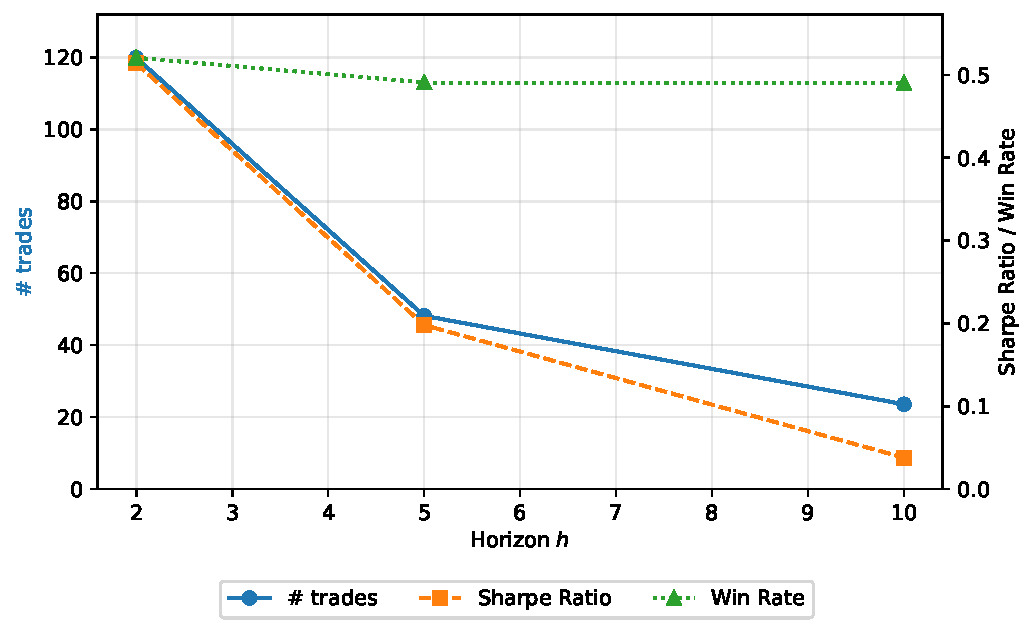
\includegraphics[width=\linewidth]{figures/fig_horizon_tradeoffs.pdf}
\caption{Mean number of trades, Sharpe ratio, and win rate by horizon over the
full grid. Predictability concentrates at the shortest horizon and decays.}
\label{fig:horizon}
\end{figure}

\begin{figure}[t]
\centering
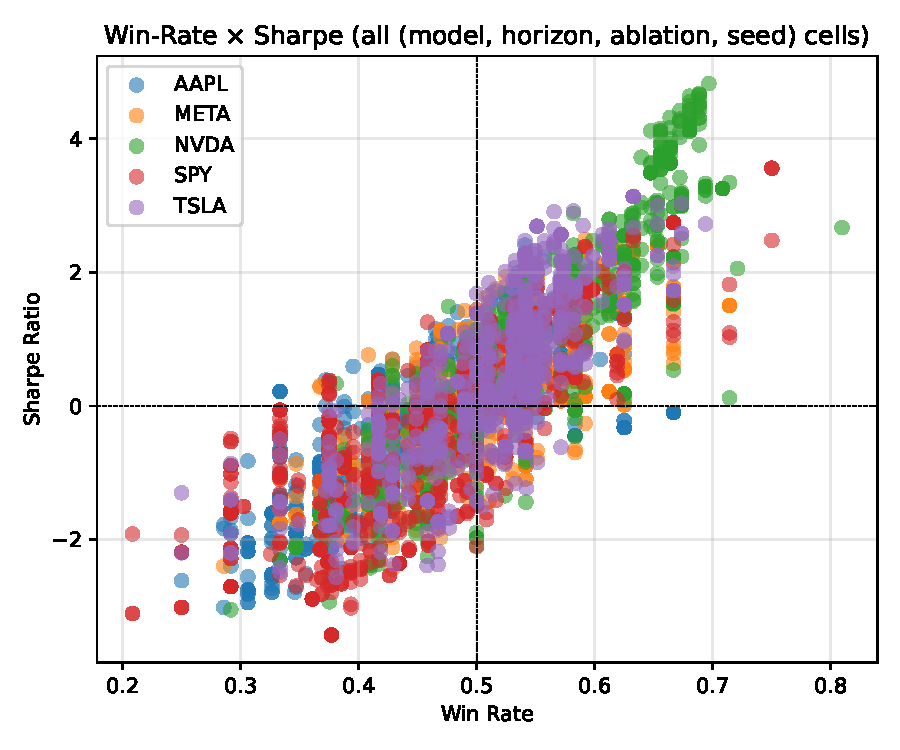
\includegraphics[width=\linewidth]{figures/fig_winrate_sharpe.pdf}
\caption{Win rate vs.\ Sharpe ratio across all task-specific runs. The two are
only weakly related: a win rate above $0.5$ does not guarantee a positive
Sharpe ratio once transaction costs and return asymmetry are accounted for.}
\label{fig:wrsharpe}
\end{figure}

\begin{figure}[t]
\centering
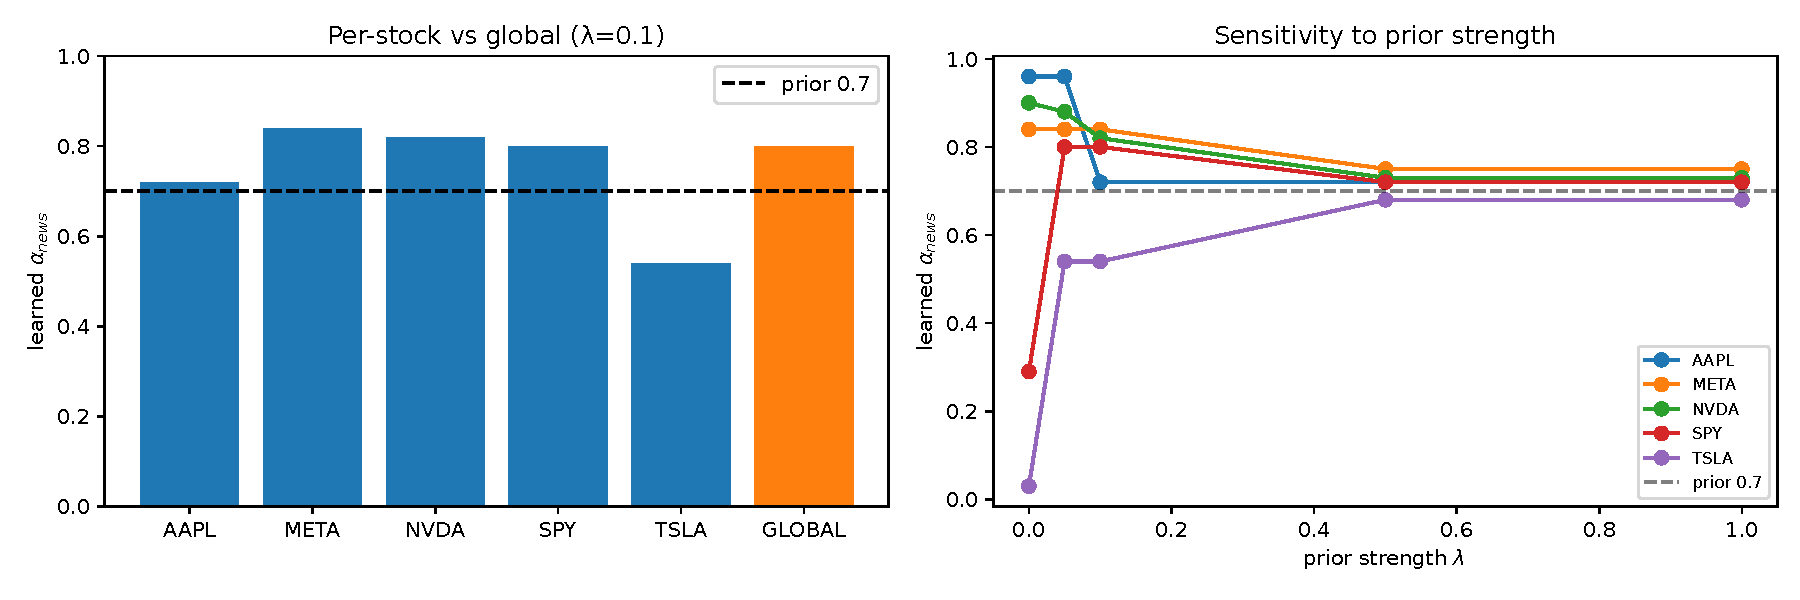
\includegraphics[width=\linewidth]{figures/fig_learned_alpha.pdf}
\caption{Learned news weight $\alpha^\star$ per stock (and global), and its
sensitivity to the prior strength $\lambda$. The weights are stable and near
the $0.7$ heuristic, but the configurations built on them still lose to
technical-only (Table~\ref{tab:ablation}).}
\label{fig:alpha}
\end{figure}

%===============================================================================
\section{Discussion}

\noindent\textbf{Why does fusion fail here?}
The proximate cause is signal: daily FinBERT-Tone sentiment correlates with
next-day returns at $|\rho|\le0.06$, with inconsistent sign across stocks. A
near-zero-signal, noisy regressor concatenated onto an informative
technical-indicator vector cannot improve a well-regularized classifier and
can degrade it---which is exactly the ordering in Table~\ref{tab:ablation}.
Aggregating thousands of documents into one daily scalar discards most of the
textual content; the scalar that remains is dominated by a persistently
positive tone (Table~\ref{tab:data}) that varies little with the next move.

\noindent\textbf{Why is this not visible in prior work?}
Two reasons. First, test-set selection (Table~\ref{tab:selbias}) manufactures
roughly $0.9$ Sharpe units regardless of features; a pipeline that quotes the
per-stock maximum will look strong whether or not sentiment helps. Second,
isolated-modality ablations are typically read on the trading metric alone,
which is dominated by variance at small trade counts; a careful paired,
multi-seed comparison---absent from most prior pipelines---tells a different
story.

\noindent\textbf{Implications.}
The contribution of this paper is therefore methodological and cautionary. The
selection-bias-free protocol of Section~\ref{sec:protocol} is inexpensive,
transferable, and, in our case, decisive: it converts an apparently strong
multimodal result---an average Sharpe ratio above two under test-set
selection (Table~\ref{tab:selbias})---into an honest finding that, here,
multimodal sentiment fusion does not help. We do not claim sentiment is universally
useless---higher-frequency text, event-level rather than daily aggregation, or
richer representations than a scalar may yet carry signal---but we do claim
that any such result must be demonstrated under an evaluation protocol that
controls for selection. We recommend that multimodal-finance studies (i)~report
a validation-locked technical-only baseline, (ii)~report paired, multi-seed
significance tests rather than per-stock maxima, and (iii)~accompany Sharpe
ratios with the Deflated Sharpe Ratio for the number of trials conducted
\cite{bailey2014dsr,bailey2016pbo}.

%===============================================================================
\section{Limitations}
\label{sec:limits}

Our study is deliberately a focused re-evaluation, and its scope bounds its
claims. (i)~\textbf{Universe:} five large-cap U.S.\ equities and a single
test year (2024); the negative result may not transfer to other regimes,
small caps, or other markets, though the selection-bias mechanism is
universal. (ii)~\textbf{Sentiment
representation:} a single daily FinBERT-Tone scalar per source; a richer
representation (document embeddings, event tags, intraday text) could carry
signal that scalar aggregation discards---testing this is the most promising
direction for future work. (iii)~\textbf{Data quality:} SPY news coverage in the
test year is only $41\%$, so SPY's sentiment ablations are partly imputed; the
conclusion is unchanged when SPY is excluded. (iv)~\textbf{Foundation models}
were run single-seed under compute limits; we therefore state their result as a
directional finding, not a precise estimate.

%===============================================================================
\section{Conclusion}

We re-evaluated the reported benefits of multimodal sentiment fusion for
short-term stock-movement prediction under a selection-bias-free protocol: an
explicit chronological split with embargo, validation-locked model and horizon
selection, multi-seed training, and paired significance testing. Across $4{,}200$ task-specific runs
and two time-series foundation models, the reported advantage of fusion did not
survive. Test-set selection alone inflates the average Sharpe ratio from
$1.40$ to $2.29$; under honest evaluation, no sentiment
configuration---including a learned reliability-weighted fusion that
generalizes the fixed 70:30 heuristic---beats a technical-indicator-only
baseline, and foundation models do not beat task-specific models. The practical
recommendation is not to abandon textual data, but to abandon optimistic
evaluation: the value of a multimodal pipeline must be demonstrated against a
validation-locked baseline with paired, multi-seed statistics. We release the
protocol, code, and processed benchmark to make that the path of least
resistance for future work.

\section*{Reproducibility}
All code, configuration files, processed per-stock features, and the
full results table are released at GitHub, together with the immutable
validation-locked selection file that all reported test numbers are read
through. A reproducibility checklist accompanies the submission.

\appendices
\section{Per-Split Dataset Statistics}
Table~\ref{tab:appendix} reports text coverage and mean news sentiment
separately for the training, validation, and test windows. The notable
irregularity is SPY news coverage in the test year ($0.41$), discussed in
Section~\ref{sec:limits}.

\begin{table}[!ht]
\caption{Text coverage by split. Train: 2020--2022; Val: 2023; Test: 2024.}
\label{tab:appendix}
\centering
\small
\setlength{\tabcolsep}{4pt}
\begin{tabular}{llccc}
\toprule
Stock & Split & News cov. & Social cov. & Mean $S^{\text{news}}$ \\
\midrule
\multirow{3}{*}{AAPL} & train & 0.988 & 1.000 & 0.489 \\
                      & val   & 1.000 & 0.992 & 0.466 \\
                      & test  & 1.000 & 0.988 & 0.350 \\
\midrule
\multirow{3}{*}{META} & train & 0.938 & 0.897 & 0.542 \\
                      & val   & 0.968 & 0.836 & 0.447 \\
                      & test  & 0.900 & 0.908 & 0.537 \\
\midrule
\multirow{3}{*}{NVDA} & train & 0.896 & 1.000 & 0.482 \\
                      & val   & 1.000 & 0.972 & 0.478 \\
                      & test  & 1.000 & 1.000 & 0.359 \\
\midrule
\multirow{3}{*}{SPY}  & train & 0.927 & 0.918 & 0.393 \\
                      & val   & 0.984 & 0.984 & 0.261 \\
                      & test  & \textbf{0.406} & 1.000 & 0.486 \\
\midrule
\multirow{3}{*}{TSLA} & train & 1.000 & 1.000 & 0.513 \\
                      & val   & 1.000 & 0.968 & 0.435 \\
                      & test  & 1.000 & 0.988 & 0.392 \\
\bottomrule
\end{tabular}
\end{table}

\balance
\bibliographystyle{IEEEtran}
\bibliography{references}

\end{document}
